%The irreducible background is very small and it is estimated using MC samples (see Fig.~\ref{fig:irr_bkg}).
The lepton identification and isolation requirements significantly suppress the background contribution, and the remnant portion of it is very small compared to the signal.
We can identify two main background components: an irreducible background from processes that produce four genuine high-$p_T$ isolated leptons, such as pp~$\to \ttbar\Z$, pp~$\to$ WWZ and pp~$\to \ttbar$~WW,  and a reducible background from processes with less than four leptons, but with jets that are identified as leptons. The irreducible background is very small and it is estimated using MC samples (see Fig.~\ref{fig:irr_bkg}).
The main background contribution arises mostly from a Z boson produced in association with jets, as well as from \ttbar, WZ and WWW + jets. This component is estimated with data analyzed in dedicated control regions and is based on the probability for particles from jet fragmentation, which satisfy predefined loose selection criteria, to also pass the final selection criteria. The procedure is described in detail in~\cite{ZZXSPaper}. In Figure~\ref{fig:red_bkg} the contribution of the reducible background is reported as a function of the 4-lepton invariant mass and the jet multiplicity, and it is estimated both from MC samples and by using the ``fake-rate'' method. The lack of statistics makes the data-driven estimate necessary.
\begin{figure}[hbtp]
  \begin{center}
   % 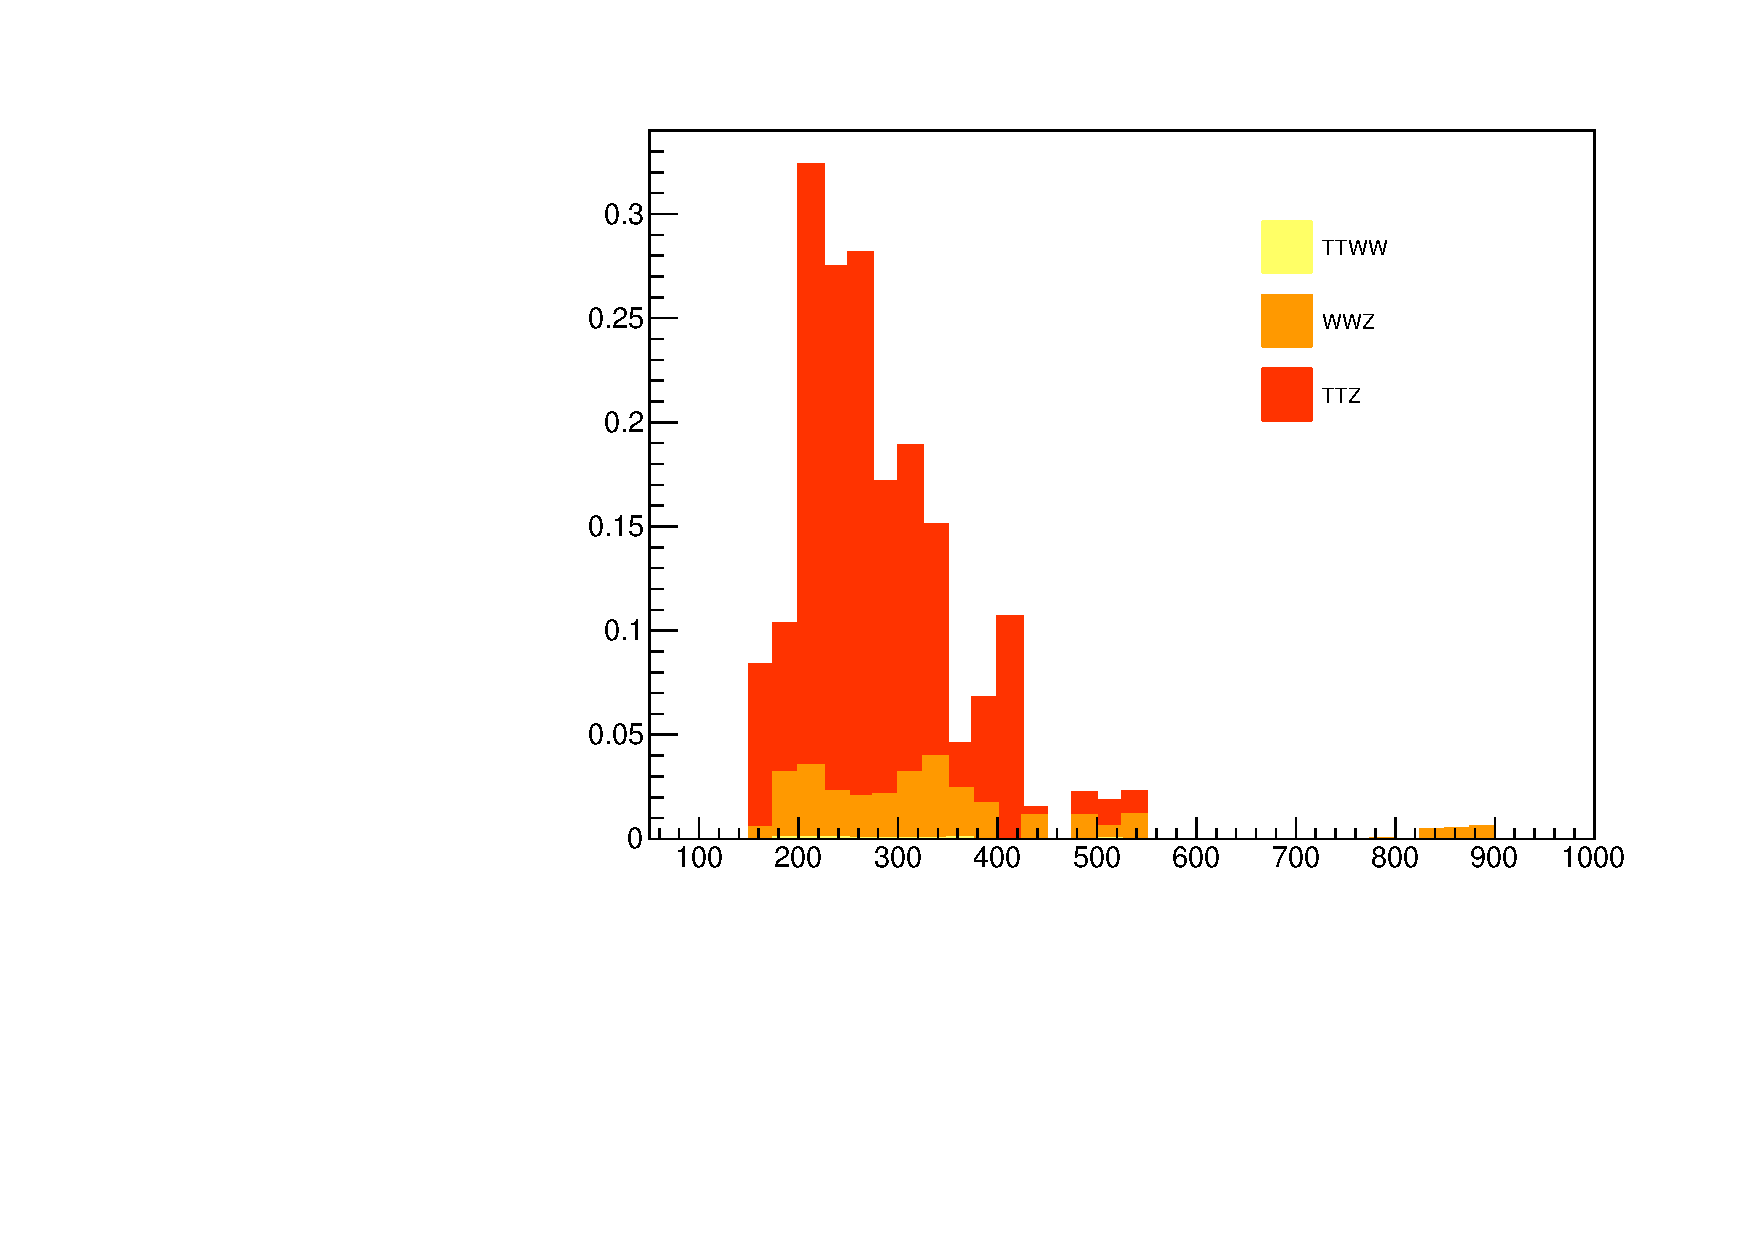
\includegraphics[width=\cmsFigWidth]{Figures/Mass_Irreducible_Bkg_MadGraphSet}
    %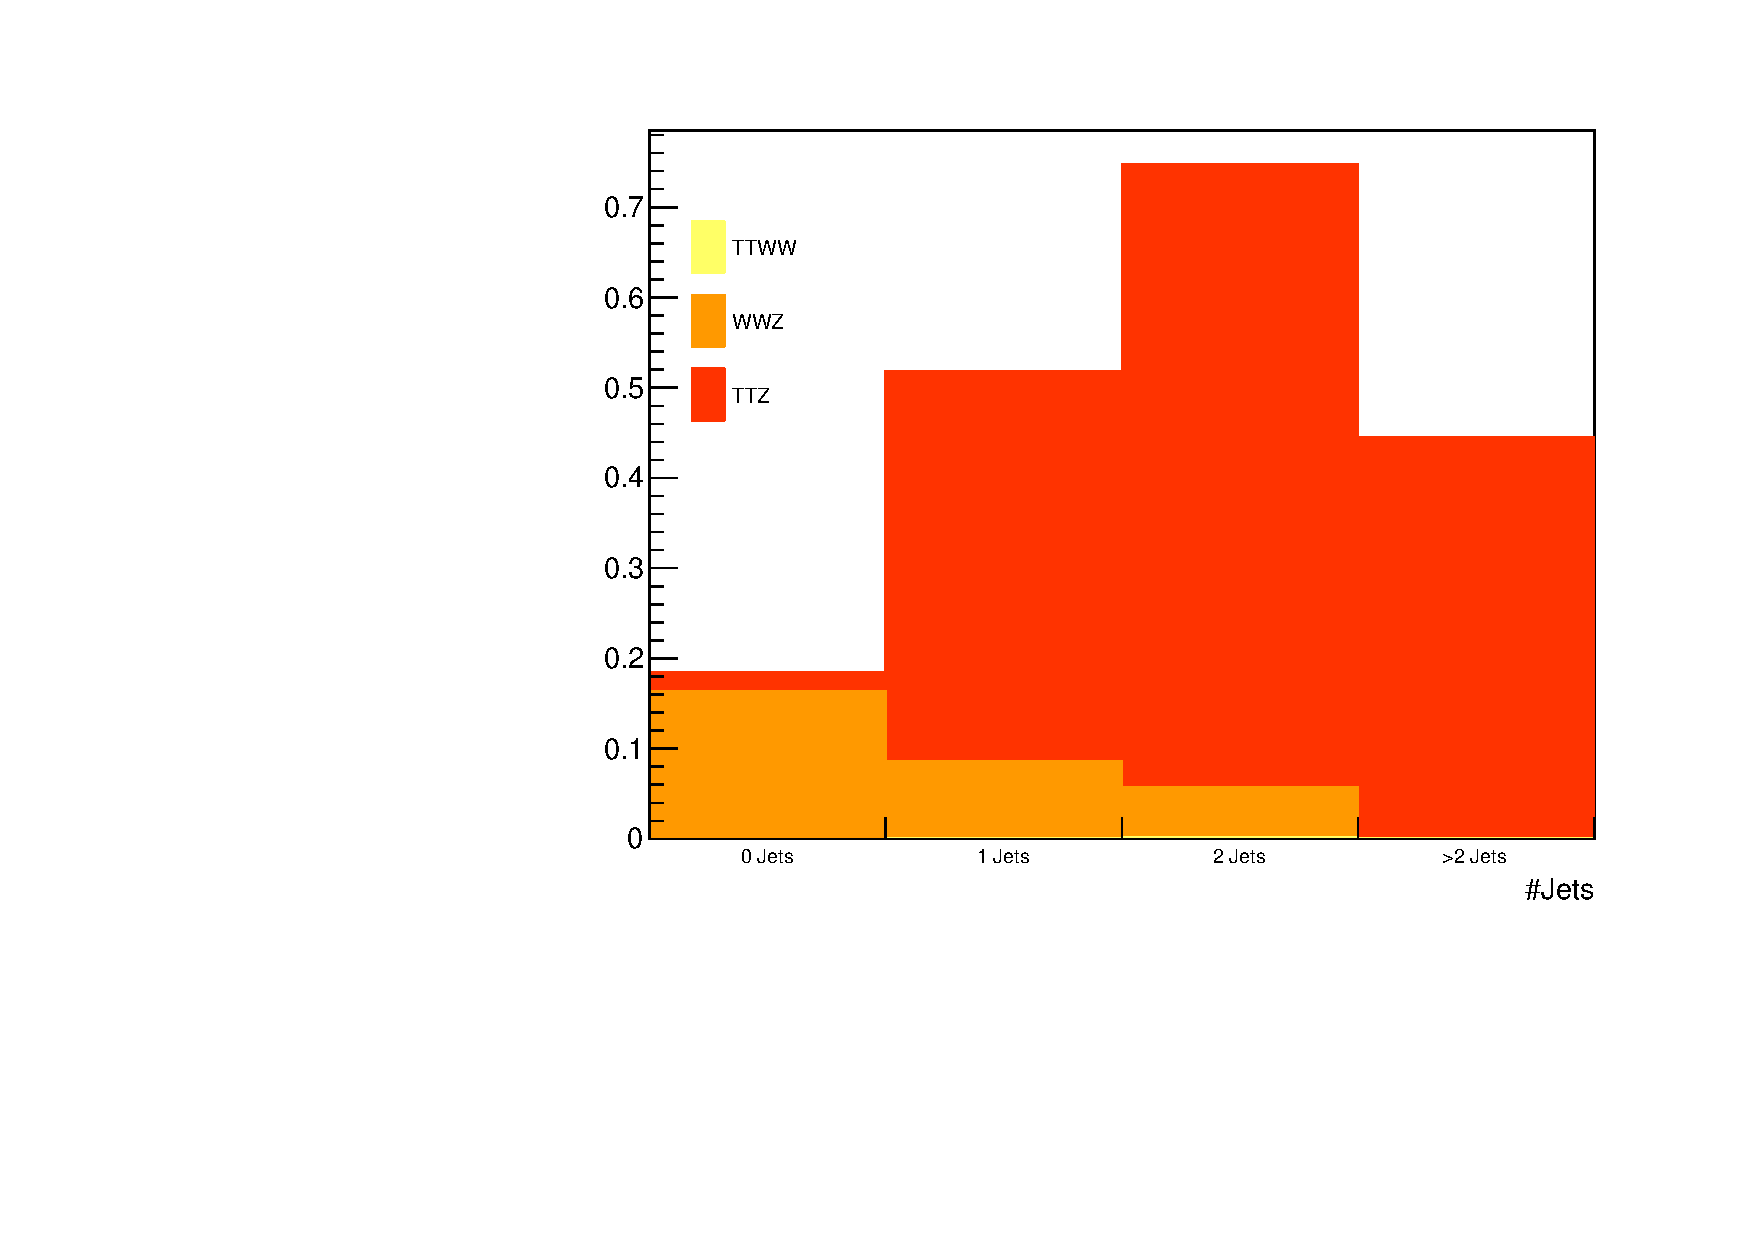
\includegraphics[width=\cmsFigWidth]{Figures/Jets_Irreducible_Bkg_MadGraphSet}
\includegraphics[width=\cmsFigWidth]{Figures/Mass_Irreducible_Bkg_pow_SR_4l}
\includegraphics[width=\cmsFigWidth]{Figures/nJets_Irreducible_Bkg_mad_SR_4l}
     \caption{Number of events of the irreducible background component in the signal region as a function of the invariant mass of the 4 lepton system (\cmsLeft) and the reconstructed number of jets produced in the event (\cmsRight).}
    \label{fig:irr_bkg}
  \end{center}
\end{figure}
\begin{figure}[hbtp]
  \begin{center}
   % \includegraphics[width=\cmsFigWidth]{Figures/Mass_Reducible_Bkg_mad_SR_4l.png}
    %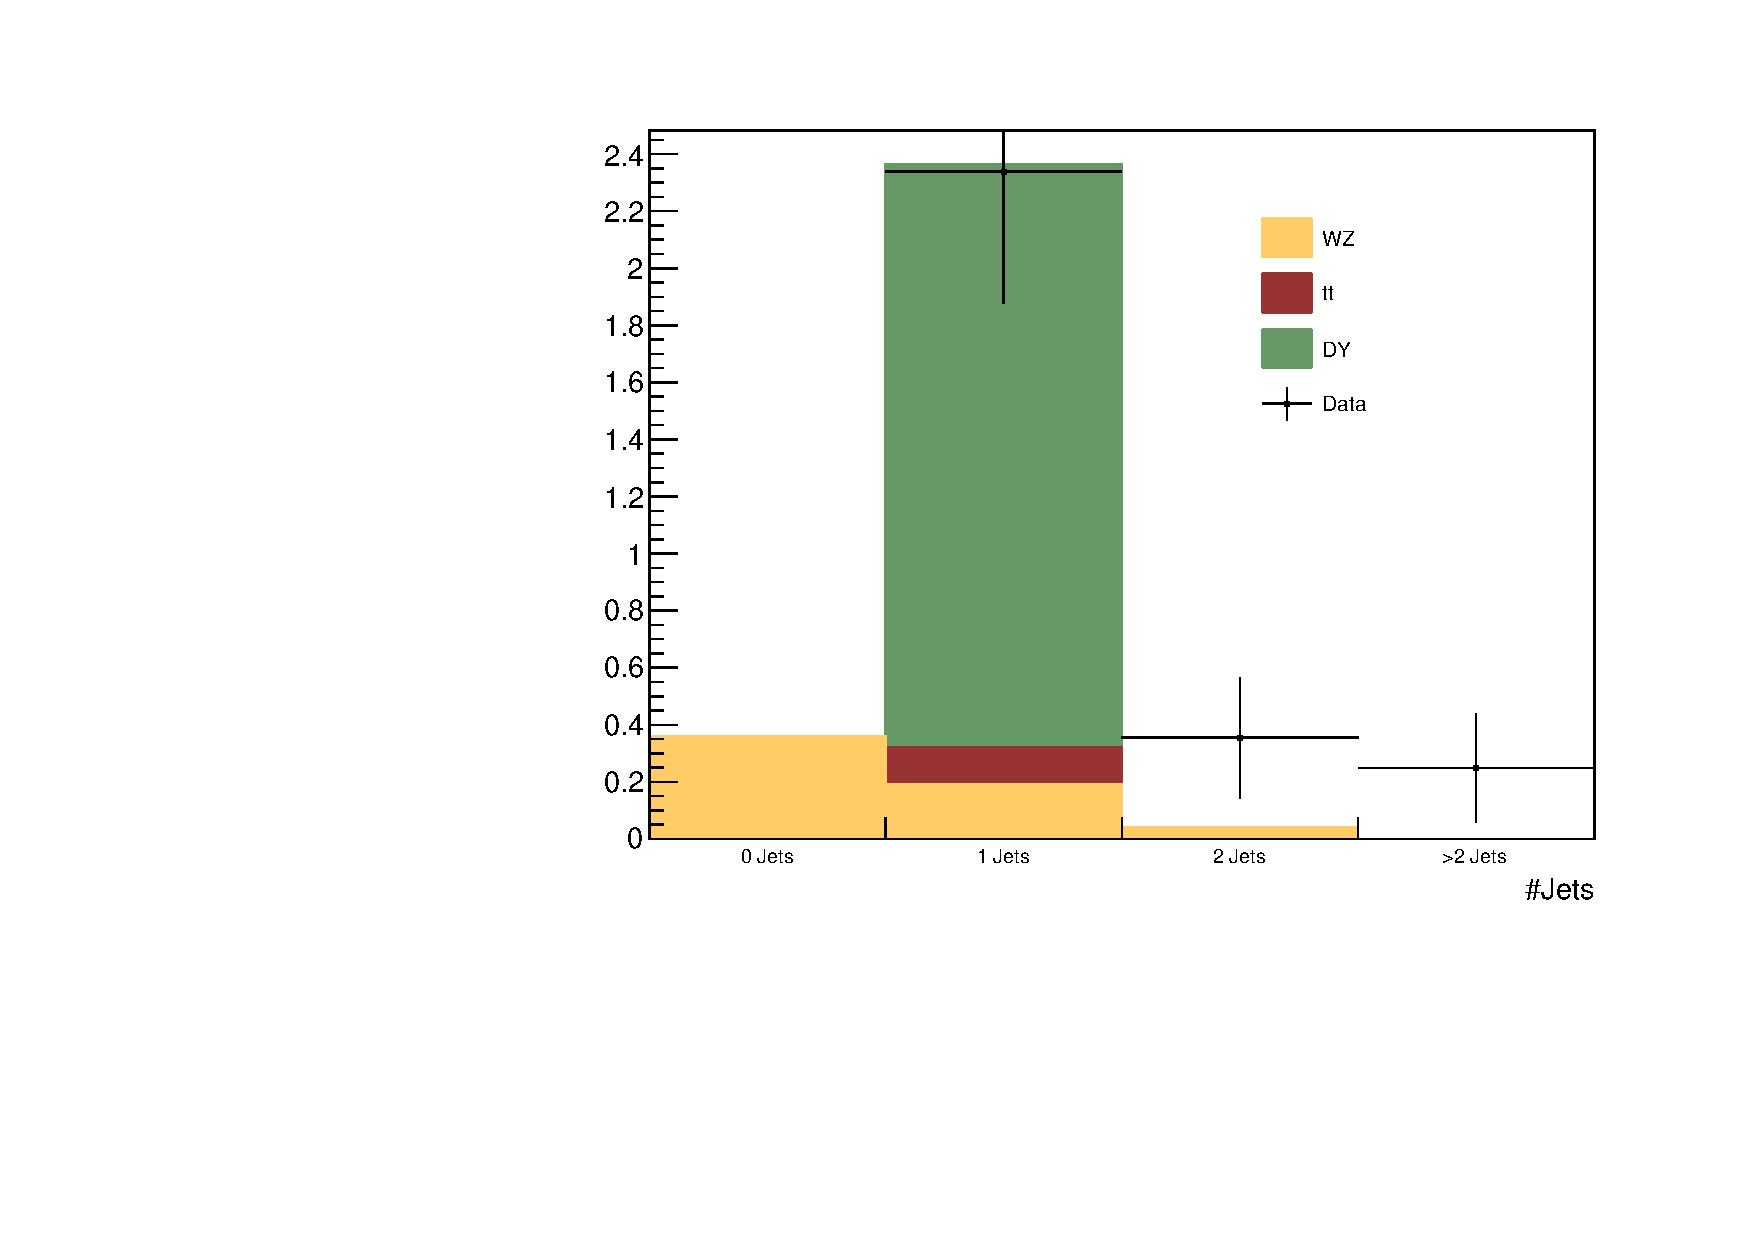
\includegraphics[width=\cmsFigWidth]{Figures/Jets_Reducible_Bkg_MadGraphSet}%FIXME 
    \includegraphics[width=\cmsFigWidth]{Figures/Mass_Reducible_Bkg_mad_SR_4l}
    \includegraphics[width=\cmsFigWidth]{Figures/nJets_Reducible_Bkg_mad_SR_4l}
     \caption{Reducible background component in the signal region as a function of the invariant mass of the 4 lepton system (\cmsLeft) and the reconstructed number of jets produced in the event (\cmsRight). Points represent the data-driven estimate, the stacked histogram represents the Monte Carlo predictions, characterized by a very poor statistics.}
    \label{fig:red_bkg}
  \end{center}
\end{figure}
%The reconstructed four-lepton invariant mass and the number of jets distributions are shown in Fig.~\ref{fig:sig_contr_Mad}.\\
%\begin{figure}[hbtp]
 % \begin{center}
  %  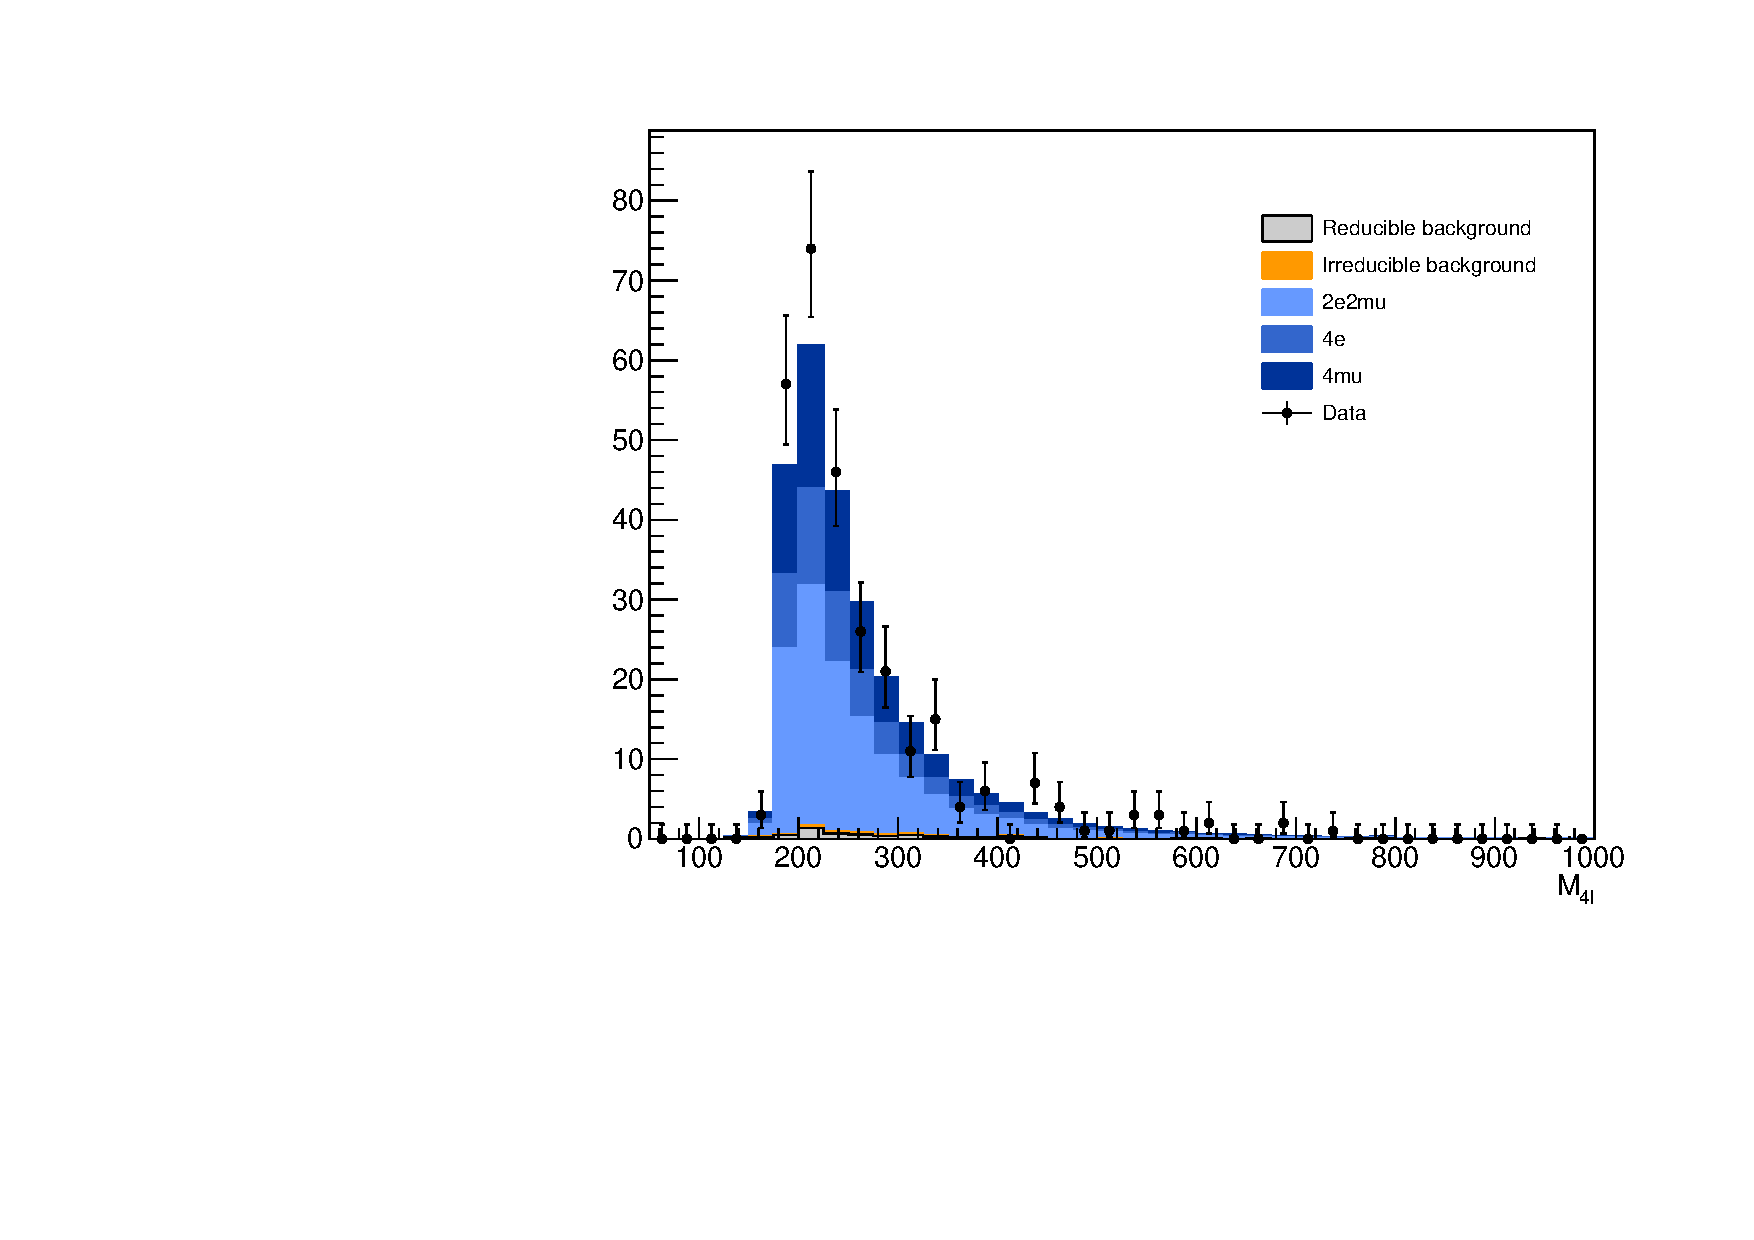
\includegraphics[width=\cmsFigWidth]{Figures/Mass_Final_State_MadGraphSet}
   % 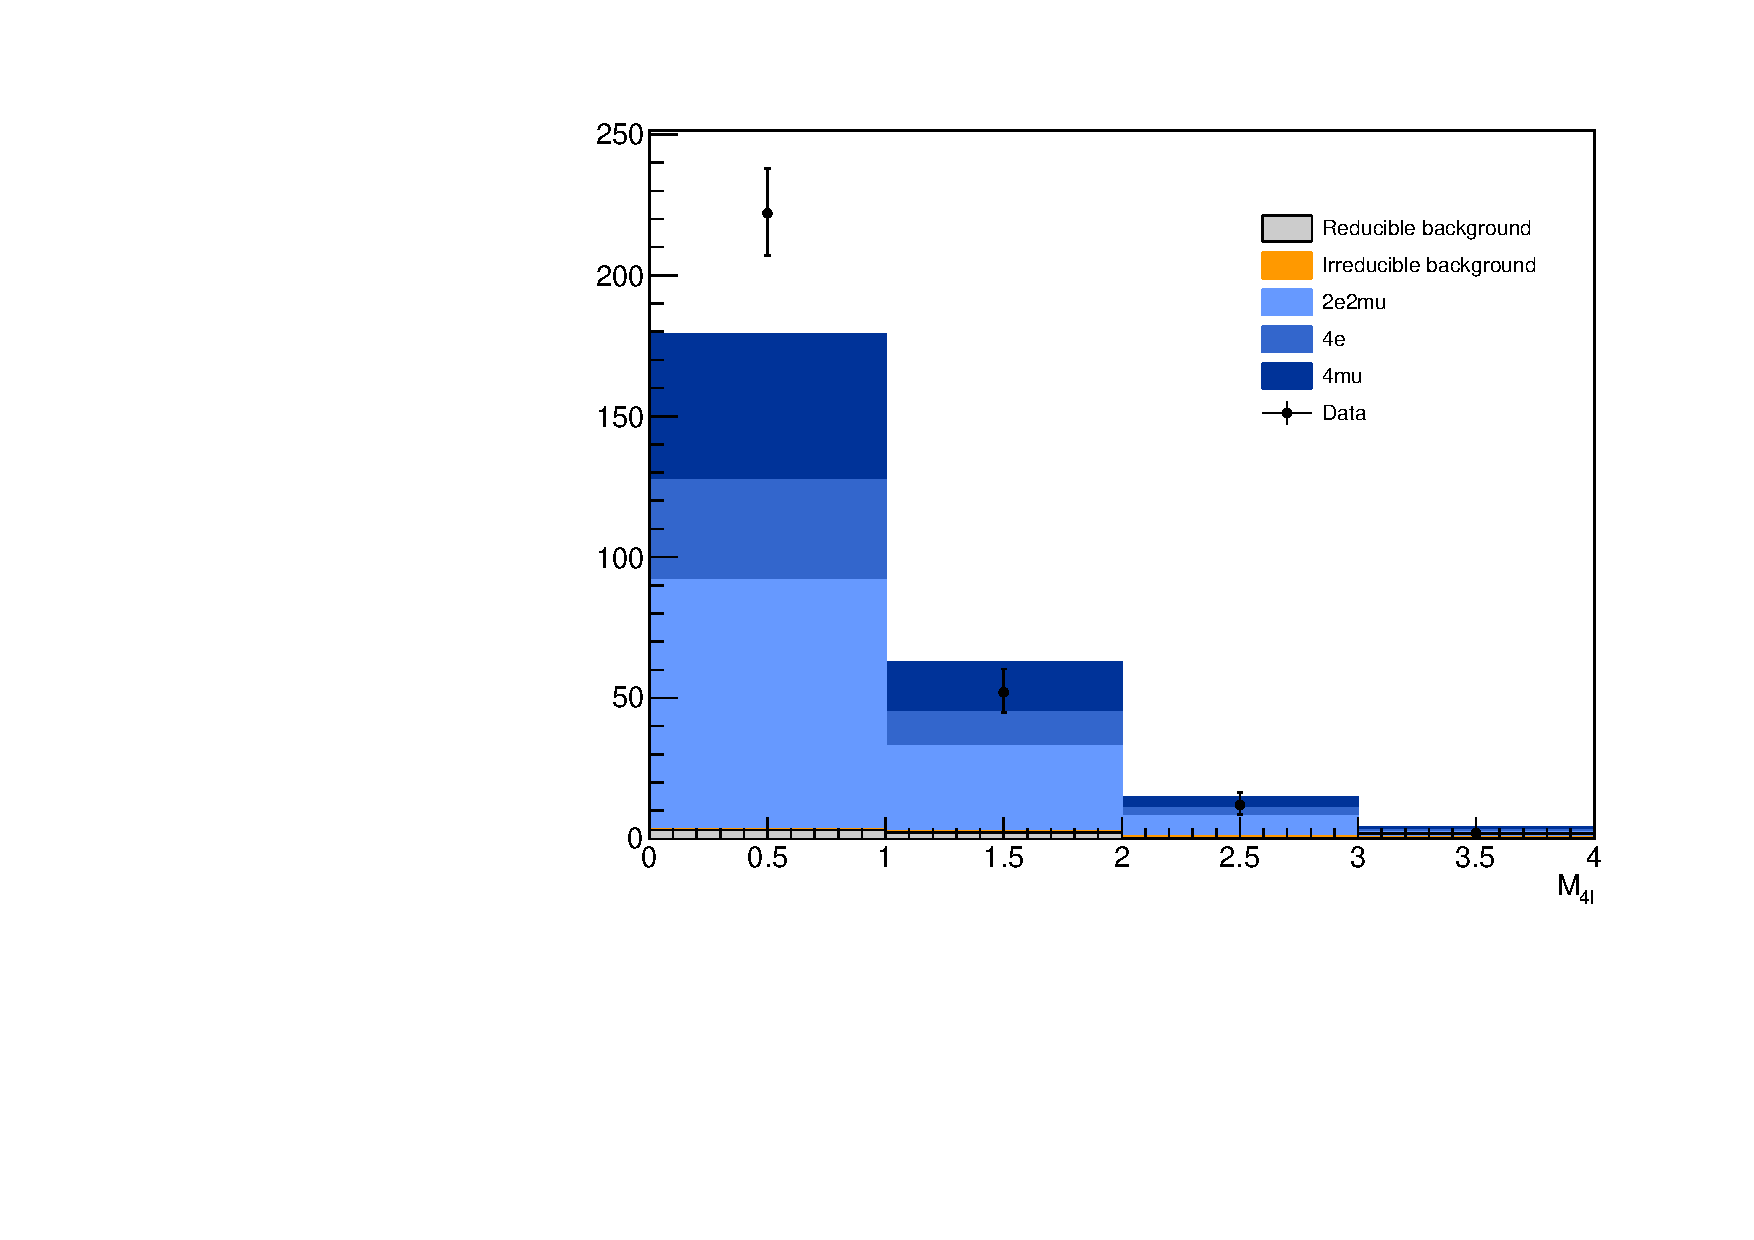
\includegraphics[width=\cmsFigWidth]{Figures/Jets_Final_State_MadGraphSet}
    % \caption{ Distribution of the reconstructed four-lepton mass (\cmsLeft). Distribution of the reconstructed number of jets produced in the event  (\cmsRight). Points represent the data, the stacked histogram represents the \texttt{MadGraph+MCFM+Phantom} predictions for $ZZ$ signal. The estimate of irreducible and reducible backgrounds is also reported.}
   % \label{fig:sig_contr_Mad}
 % \end{center}
%\end{figure}
